% !TEX program = XeLaTeX
% !TEX encoding = UTF-8
\documentclass[UTF8,nofonts]{ctexart}
\setCJKmainfont[BoldFont=FandolSong-Bold.otf,ItalicFont=FandolKai-Regular.otf]{FandolSong-Regular.otf}
\setCJKsansfont[BoldFont=FandolHei-Bold.otf]{FandolHei-Regular.otf}
\setCJKmonofont{FandolFang-Regular.otf}

\usepackage{url}
\usepackage{cancel}
\usepackage{xspace}
\usepackage{graphicx}
\usepackage{multicol}
\usepackage{multirow}
\usepackage{subfig}
\usepackage{amsmath}
\usepackage{amssymb}
\usepackage[a4paper, width=186mm, top=18mm, bottom=18mm, includeheadfoot]{geometry}
\usepackage{booktabs}
\usepackage{array}
\usepackage{verbatim}
\usepackage{caption}
\usepackage{natbib}
\usepackage{booktabs}
\usepackage{float}
\usepackage{pdflscape}
\usepackage{mathtools}
\usepackage[usenames, dvipsnames]{xcolor}
\usepackage{afterpage}
\usepackage{pgf}
\usepackage{tikz}
\usepackage{dirtree}
\usepackage[style=american]{csquotes}
\usepackage{amsfonts}
\usepackage{tikz}
\usepackage{tkz-graph}
\usetikzlibrary{arrows,decorations.pathmorphing,automata,positioning,backgrounds,fit,shapes.symbols,chains,intersections}
\usepackage{scrextend}
\addtokomafont{labelinglabel}{\sffamily}

\newtheorem{definition}{Definition}[section]
\newtheorem{theorem}{Theorem}[section]
\newtheorem{lemma}{Lemma}
\newtheorem{proof}{Proof} [section]

\usepackage[toc, page, title, titletoc, header]{appendix}
\usepackage{marginnote}
\usepackage{tablefootnote}

\renewcommand\abstractname{Abstract}


\usepackage{perpage} %the perpage package
\MakePerPage{footnote} %the perpage package command

\usetikzlibrary{shapes.geometric}%
\usepackage{color}
%\usepackage[pages=some, placement=top]{background}
\usepackage{eso-pic}
\usepackage[final]{pdfpages}

%\includepdf[pages=1]{cover}
\hyphenpenalty=750

\title{\textbf{Vite:}\textbf{一个异步高性能的通用去中心化应用平台}}
\author{
  刘春明\\
  \texttt{charles@vite.org}\\
  \and
  	王东\\
  	\texttt{daniel@loopring.org}\\
  	\and
  	伍鸣\\
  	\texttt{woo@vite.org}\\
 }

\makeatletter
\def\CTEX@section@format{\Large\bfseries}
\makeatother

\makeatletter
\newenvironment{tablehere}
 {\def\@captype{table}}
 {}
 
\newenvironment{figurehere}
 {\def\@captype{figure}}
 {}
\makeatother

\begin{document}

\maketitle

\begin{abstract}
摘要。
\end{abstract}

\begin{multicols}{2}

\section{简介}
\subsection{定义}

一个通用去中心化应用平台,可以支持一组智能合约,每个智能合约都是一个拥有独立状态以及不同操作逻辑的交易状态机,它们之间可以通过消息传递的方式进行通信。

从整体上,这个系统是一个交易状态机。系统的状态$\boldsymbol{s}\in\boldsymbol{S}$也称为世界状态,是由每一个独立账户的状态构成的。一个能够引起世界状态改变的事件称为交易。更形式化的定义如下:

\begin{definition}[交易状态机] \label{def-fsm}
一个交易状态机是一个四元组: $(\boldsymbol{T},\boldsymbol{S},\boldsymbol{g},\boldsymbol{{\delta}})$,其中,$\boldsymbol{T}$是交易的集合,$\boldsymbol{S}$是状态的集合,$\boldsymbol{g} \in \boldsymbol{S}$为初始状态,也称为“创世块”,$\boldsymbol{{\delta}:\boldsymbol{S}\times\boldsymbol{T}\rightarrow\boldsymbol{S}}$是状态转移函数。
\end{definition}

这种交易状态机的语义是一个离散迁移系统,定义如下:
\begin{definition}[交易状态机的语义] \label{def-semantics}
一个交易状态机$(\boldsymbol{T},\boldsymbol{S},\boldsymbol{s_{0}},\boldsymbol{{\delta}})$的语义是一个离散迁移系统: $(\boldsymbol{S},\boldsymbol{s_{0}},\boldsymbol{\rightarrow})$。$\boldsymbol{\rightarrow} \in \boldsymbol{S}\times\boldsymbol{S}$是迁移关系,
\end{definition}

同时,去中心化应用平台是一个分布式系统,具有最终一致性。通过某种共识算法,节点间可以就最终的状态达成一致。在现实场景中,智能合约的状态中保存的是一个去中心化应用的全部数据,体积比较大,无法在节点间传输。因此,节点间需要通过传递一组交易,来达成最终状态的一致。我们将这样的一组交易组织成某种特定的数据结构,通常称之为账本。

\begin{definition}[账本] \label{def-ledger}
账本是由一组交易构成的,具有递归构造的抽象数据类型,定义如下:
$$
\left\{\begin{matrix}
l = \Gamma(T_{t})\\ 
l = l_{1} + l_{2}
\end{matrix}\right.
$$
其中,$T_{t} \in 2^{T}$,表示一组交易, $\Gamma \in 2^{T} \rightarrow L$,表示通过一组交易构造一个账本的函数,$L$是账本的集合,$\boldsymbol{+}: L \times L \rightarrow L$,表示将两个子账本合并成一个账本的操作。
\end{definition}

需要注意的是,在此类系统中,账本通常用来表示一组交易,而不是一个状态。在比特币\cite{nakamoto2008bitcoin}和以太坊\cite{wood2014ethereum}中,账本是一个区块链结构,其中交易是全局有序的。修改账本中的一个交易,需要重新构造账本中的一个子账本,从而提高了篡改交易的成本。

根据同一组交易,可以构造出不同的有效账本,但它们所表示的交易顺序不同,因此可能会导致系统进入不同的状态。当这种情况发生时,通常称账本发生了“分叉”。
\begin{definition}[分叉] \label{def-fork}
$T_{t},{T_{t}}' \in 2^{T}$,$l=l_{1} + \Gamma_{1}(T_{t})$, ${l}'=l_{1}+\Gamma_{2}({T_{t}}')$,且$l \neq {l}'$,则称$l$和${l}'$是分叉账本。 
\end{definition}

根据交易状态机的语义,我们可以很容易的证明,从一个初始状态开始,如果账本不分叉,则每个节点最终会进入相同的状态。那么,如果接收到分叉的账本,就一定进入不同的状态吗?这取决于账本中交易的内在逻辑,以及账本如何组织交易之间的偏序。现实中,经常会出现一些满足交换律的交易,却因为账本设计的问题,频繁的引起分叉。当系统从一个初始状态出发,接收两个分叉的账本,最终进入同一状态,我们称这两个账本为伪分叉账本。

\begin{definition}[伪分叉] \label{def-falsefork}
有初始状态$s_{0} \in S$,账本$l_{1},l_{2} \in L$,$s_{0}\overset{l_{1}}{\rightarrow}s_{1}, s_{0}\overset{l_{2}}{\rightarrow}s_{2}$。若$l_{1} \neq l_{2}$,且$s_{1}=s_{2}$,则称这两个账本$l_{1} ,l_{2}$为伪分叉(false fork)账本。
\end{definition}

一个设计良好的账本,应该尽量降低伪分叉发生的概率。

当分叉发生时,每个节点都需要从多个分叉的账本中选择一个,为确保状态的一致性,这些节点需要采用同一个算法完成选择,这个算法称为共识算法。

\begin{definition}[共识算法] \label{def-consensus}
共识算法是一个函数,它接收一个账本的集合,返回其中唯一一个账本:
$$\Phi: 2^{L} \rightarrow L$$
\end{definition}

共识算法是系统设计的一个重要内容,一个好的共识算法应该具有较高的相交速度(high convergence speed),减少共识在不同分叉间摇摆,并对恶意攻击具有较高的防范能力。

\subsection{当前进展}
以太坊\cite{buterin2017ethereum}率先实现了这样一个系统。
在以太坊的设计中,世界状态的定义是:$S = \Sigma^{A}$,是由每个账户$a \in A$与该账户的状态$\sigma_{a} \in \Sigma$构成的映射。因此,以太坊的状态机中任何一个状态都是全局的,这表示一个节点在每个时刻都可以获取任何一个账户的状态。

以太坊的状态转移函数$\delta$,是由一组程序代码来定义的,每组代码被称为一个智能合约。以太坊定义了一个图灵完备的虚拟机,称为EVM,运行在其上的指令集称为EVM代码。用户可以通过一种语法类似于javascript的程序语言Solidity来开发智能合约,并编译成EVM代码,部署到以太坊上\cite{dannen2017introducing}。一旦智能合约部署成功,就相当于定义了该合约账户$a$收到一个交易后的状态转移函数$\delta_{a}$。
EVM目前在此类平台中被广泛使用,但它也存在一些问题。例如,缺少库函数支持,安全性问题突出等。

以太坊的账本结构是区块链\cite{nakamoto2008bitcoin},区块链由区块构成,每一个区块中包含一组交易的列表,后一个区块引用前一个区块的hash,构成一个链状结构。
\begin{equation}
\Gamma(\lbrace t_{1}, t_{2},...\vert t_{1}, t_{2},... \in T \rbrace) = (..., (t_{1}, t_{2},...)) 
\end{equation}
这个结构的最大好处是有效的防止交易被篡改,但由于它维护的是所有交易的全序,任何两个交易交换顺序,都会生成一个新账本,也造成这种结构具有较高的分叉概率。事实上,在这个定义下,交易状态机的状态空间被看作一棵树:初始状态是根节点,不同的交易顺序代表不同的路径,叶子节点是最终状态。现实的情况下,大量叶子节点的状态是相同的,这就造成了大量的伪分叉。

以太坊的共识算法$\Phi$称为PoW,该算法率先在比特币协议中提出\cite{nakamoto2008bitcoin}。PoW算法依赖于某个易于验证但难于求解的数学问题,例如,根据一个hash函数$h:N \rightarrow N$,求解$x$,使$h(T+x) \geq d$,$d$是一个给定的数,称为难度,T是区块中包含的交易列表的二进制表示。在区块链的每个区块中,都会包含这类问题的一个解。将全部区块的难度加起来,就是一个区块链账本的总难度:
\begin{equation}
D(l) = D(\sum_{i} l_{i}) = \sum_{i} D(l_{i})
\end{equation}

因此,在从分叉中选择正确账本的时候,只要选择总难度最高的分叉即可:
\begin{equation}
 \Phi (l_{1}, l_{2}, ..., l_{n}) = l_{m} \text{ where } D(l_{m}) = max(D(l_{i}))
\end{equation}

PoW共识算法具有较好的安全性,迄今为止在比特币和以太坊中运行得很好。但这个算法有两个主要问题,第一是求解数学难题需要消耗大量计算资源,造成能源浪费;第二是该算法相交速度较慢,因而影响了系统整体的吞吐。目前,以太坊整体的TPS只有15左右,完全无法满足去中心化应用的需求。

\subsection{改进方向}
在以太坊诞生之后,以太社区和其他一些同类项目开始从不同方向对系统加以改进。从系统的抽象模型来看,可以改进的方向主要包括以下几个:
\begin{itemize}
	\item 改进系统状态$\boldsymbol{S}$	
	\item 改进状态迁移函数$\boldsymbol{\delta}$	
	\item 改进账本结构$\boldsymbol{\Gamma}$
	\item 改进共识算法$\boldsymbol{\Phi}$
\end{itemize}

\subsubsection{改进系统状态}
对系统状态的主要改进思路是将全局的世界状态局部化,每个节点不再关心全部交易和状态转移,只维护整个状态机的一个子集。这样集合$S$和集合$T$的势都大为缩减,从而提高了系统扩展性。此类系统包括:Cosmos\cite{cosmos},Aelf\cite{aelf},PChain等。

从本质上讲,此类基于侧链的方案牺牲了状态的全局性,以换取系统的扩展性。这使得每个运行在其上的dApp的去中心化程度都被削弱——一个智能合约的交易历史不再被全网每一个节点保存,而只被一部分节点保存。
除此之外,跨合约交互也会成为此类系统的瓶颈。例如,Cosmos中,不同的Zone交互,需要通过一个共同的链Hub来完成\cite{cosmos}。

\subsubsection{改进状态迁移函数}
一些项目立足于改进EVM,提供更为丰富的智能合约编程语言。例如,RChain	定义了一种基于$\pi$演算的智能合约语言Rholang;NEO中的智能合约称为NeoContract,可以用Java,C\# 等主流编程语言开发;EOS使用C/C++来编程。

\subsubsection{改进账本结构}
账本结构的改进方向是构造等价类,将多个交易全局有序的线性账本规约为一个只记录部分偏序关系的非线性账本,这种非线性账本结构是一个DAG(有向无环图)。目前,Byteball\cite{byteball},IOTA\cite{iota},Nano\cite{nano}等项目基于DAG的账本结构实现了加密货币功能。也有一些项目在尝试利用DAG实现智能合约,但迄今为止在这个方向上的改进还在探索中。

\subsubsection{改进共识算法}
共识算法的改进大部分是为了提高系统的吞吐,主要方向是抑制伪分叉的产生。下面我们讨论伪分叉与哪些因素有关。

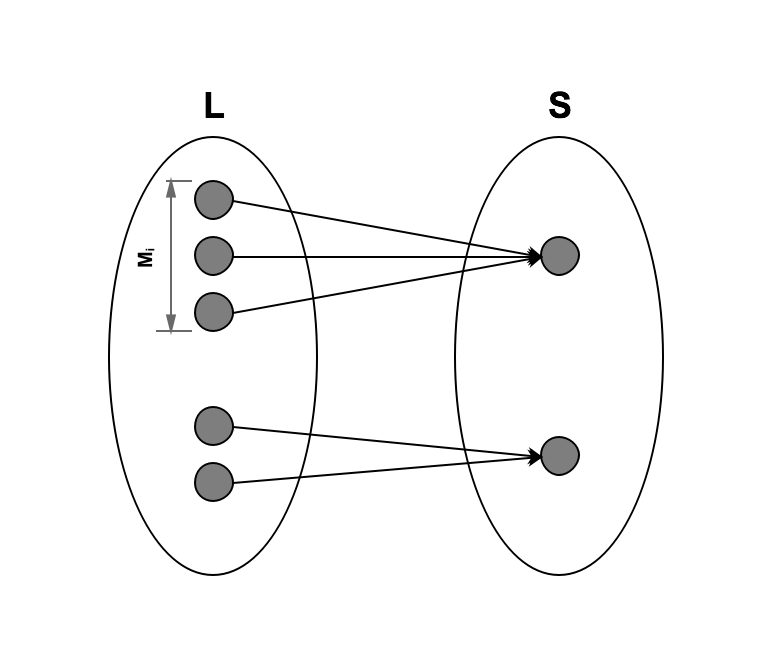
\includegraphics[width=.8\linewidth]{image/falsefork.png}

如图所示,$L$是针对某个交易集合所有可能的分叉账本的集合,$S$是以不同顺序执行这一组交易,所能到达的状态的集合。根据定义 \ref{def-fork},映射$f: L \rightarrow S$是一个满射;而根据定义 \ref{def-falsefork},这个映射不是单射。下面我们来计算伪分叉的概率:

假设共有$C$个用户有权生产账本,$M = \vert L \vert$,$N = \vert S \vert$,$M_{i} = \vert L_{i} \vert$, 其中,$L_{i} = \lbrace l \vert f(l) = s_{i}, s_{i} \in S \rbrace$。
则伪分叉概率为:
\begin{equation}
P_{ff} = \sum_{i=1}^{N}\left ( \frac{M_{i}}{M} \right )^{C} - \frac{1}{M^{C-1}}
\end{equation}

从这个公式可以看出,为了降低伪分叉概率,可以有两种途径:
\begin{itemize}
	\item 在账本集合$L$上建立等价关系,对其划分等价类,构造分叉更少的账本
	\item 限制有权生产账本的用户,从而减少$C$
\end{itemize}

第一种途径是Vite设计的重要方向,后文将详细论述;第二种途径现在已被多种算法所采用。在PoW算法中,任何用户都有权生产区块;而PoS算法将生产区块的权力限制在那些拥有系统权益的用户中;DPoS算法\cite{dpos}将有权生产区块的用户进一步限制在一组代理节点范围内。
	
目前,通过改良共识算法,已经产生出一些比较有影响力的项目。例如,Cardano采用了一种PoS算法,称为Ouroboros,文献\cite{bernardo2017ouroboros}对该算法相关性质给出了严格证明;EOS采用了DPoS算法,通过快速生产区块,提高系统的吞吐;Qtum\cite{dai2017smart}的共识算法也是一种PoS算法;RChain采用的Casper算法也是一种PoS算法。

还有一些其他项目在共识算法的改进上提出了自己的方案。NEO采用了一种BFT算法,称为dBFT;Cosmos采用了一种称为Tendermint\cite{tendermint}的算法。

\section{账本}
\subsection{概述}
账本的作用主要是为了确定交易之间的顺序,交易的顺序会影响以下两个方面:
\begin{itemize}
	\item \textbf{状态一致性:} 由于系统的状态不是一个CRDT(Conflict-free replicated data types)\cite{crdt},因此,交易不都是可交换的,不同的交易执行顺序可能会导致系统进入不同的状态。
	\item \textbf{hash有效性:} 账本中,交易会被打包成区块,区块中包含互相引用的hash。交易的先后顺序会影响账本中hash引用的连通性。这种影响的范围越大,篡改交易的成本就越大。这是因为,改变任何一个交易,都必须重建所有直接或间接引用该交易的区块的hash。
\end{itemize}

而账本的设计也有两个主要目标:

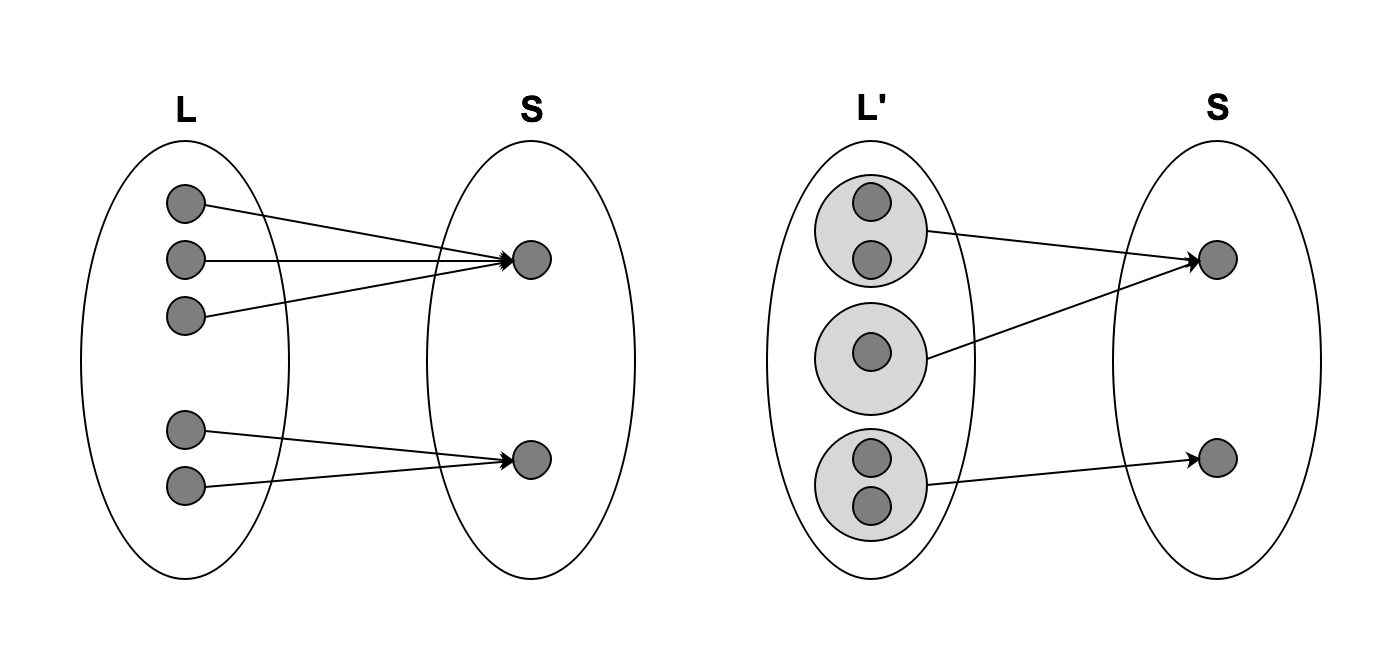
\includegraphics[width=.9\linewidth]{image/ledger-merge.png}

\begin{itemize}
	\item \textbf{降低伪分叉率:} 如前文讨论,降低伪分叉率可以通过建立等价类,尽量将导致系统进入同一状态的一组账本合并成一个账本来实现。如上图,根据伪分叉率公式可以算得,左图的账本伪分叉率$P_{ff}=\left (  \frac{3}{5} \right )^{C} + \left (  \frac{2}{5} \right )^{C} - \frac{1}{5^{C-1}}$;而合并账本空间后,右图的伪分叉率为${P_{ff}}'=\left (  \frac{2}{3} \right )^{C} + \left (  \frac{1}{3} \right )^{C} - \frac{1}{3^{C-1}}$。可知当$C > 1$,${P_{ff}}' < P_{ff}$。也就是说,我们应尽量减小账本中交易之间的偏序关系,允许更多的交易之间的顺序可交换。
	\item \textbf{防篡改:} 当账本$l$中一个交易$t$被修改,账本的两个子账本$l = l_{1} + l_{2}$中,子账本$l_{1}$不受影响,而子账本$l_{2}$中的hash引用需要重建,以构成一个新的有效账本${l}' = l_{1} + {l_{2}}'$。受影响的子账本$l_{2} = \Gamma(T_{2}),T_{2} = \lbrace x \vert x \in T, x > t \rbrace $。由此可见,想提高篡改交易的成本,需要在账本中尽量多的维护交易之间的偏序关系,以扩大篡改的影响范围$\vert T_{2} \vert$。
\end{itemize}

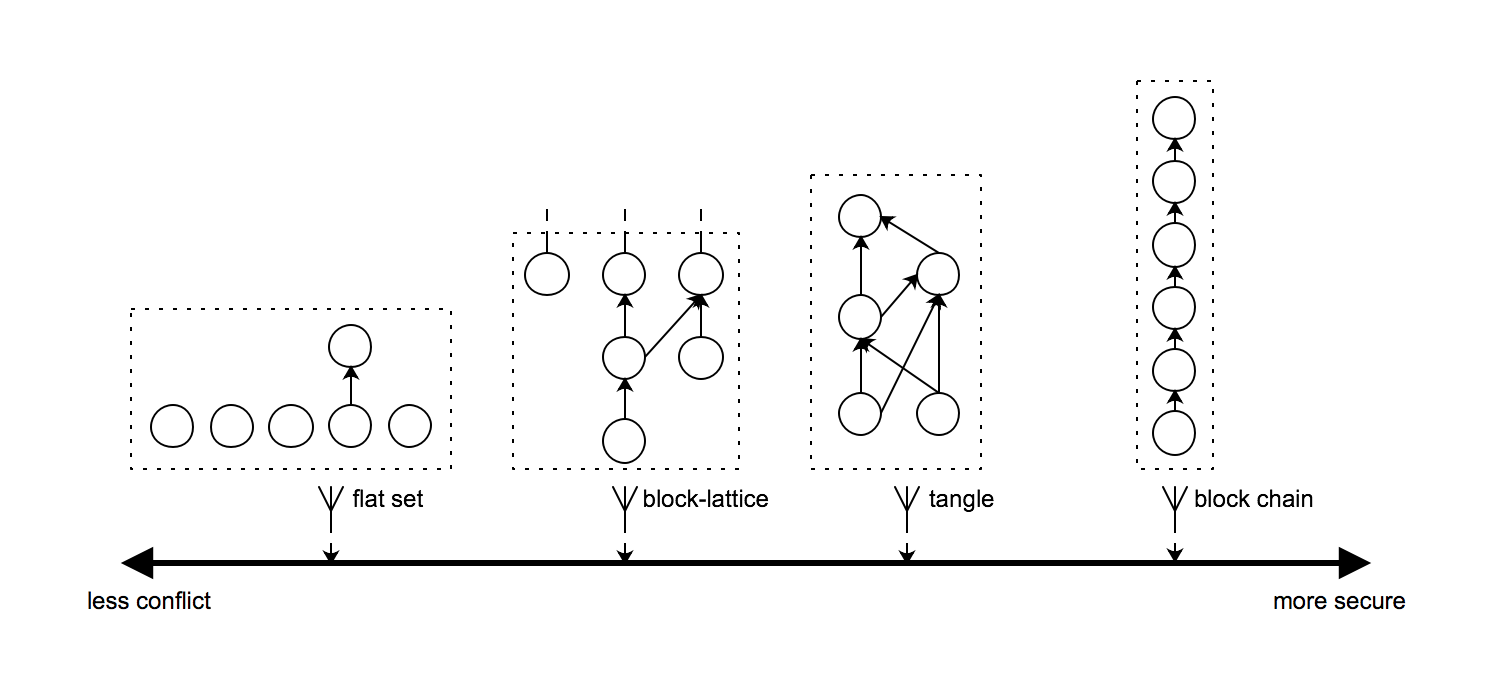
\includegraphics[width=\linewidth]{image/ledger-compare.png}

显然,以上两个目标是互相矛盾的,在设计账本结构时必须作出必要的权衡取舍。由于账本维护的是交易之间的偏序,因此它本质上是一个偏序集(poset)\cite{poset},如果用哈斯图(Hasse diagram)\cite{hasse}来表示,在拓扑上就是一个DAG。

上图对比了几种常见的账本结构,靠近左侧的账本维护更少的偏序关系,哈斯图显得比较扁平,具有更低的伪分叉率;靠近右侧的账本维护更多的偏序关系,哈斯图比较细长,具有更高的防篡改特性。

图中,最左侧的是一种中心化系统中常见的基于集合的结构,没有任何防篡改特性;最右侧则是典型的区块链账本,具有最好的防篡改特性;而介于二者中间的是两种DAG账本,左侧的是Nano采用的block-lattice账本\cite{nano},右侧是IOTA采用的tangle账本\cite{iota}。从特性上看,block-lattice维护了更少的偏序关系,更适合作为高性能去中心化应用平台的账本结构。但由于它的防篡改特性较差,会产生安全隐患,因此,迄今为止,除了Nano采用了该结构之外,还没有其他项目采用。

为了追求高性能,Vite采用该账本结构。同时,通过引入一种额外的链式结构Snapshot Chain,并且改进了共识算法,成功的弥补了block-lattice安全性方面的不足,后文将详细论述这两个改进。

\subsection{前置约束}
首先,我们来看一下采用这种账本结构对状态机模型的前置要求。这种结构本质上是将整个状态机看作是一组独立的状态机的组合,每个账户对应一个独立的状体机,每个交易只影响一个账户的状态。在账本,对所有交易按账户分组,并把同一账户的交易组织成一条链。因此,我们对Vite中的状态$S$和交易$T$做出如下限制:

\begin{definition}[交易的单自由度约束]
系统状态$s \in S$,是由每个账户的状态$s_{i}$构成的向量$s=(s_{1}, s_{2},...,s_{n})$。对于$\forall t_{i} \in T$,执行交易$t_{i}$后,系统状态发生如下转移:$({s_{1}}',..., {s_{i}}',...,{s_{n}}') = \sigma(t_{i}, (s_{1},..., s_{i},...,s_{n}))$,需满足:${s_{j}}'=s_{j} , j \neq i$。该约束称为交易的单自由度约束。
\end{definition}

直观上,一个单自由度的交易只会改变一个账户的状态,不会影响系统中其他账户的状态。在状态空间向量所在的多维空间中,执行一次交易,系统状态只会沿平行于某个坐标轴的方向移动。请注意,这个定义要比比特币、以太坊等模型中的交易定义更为严格,比特币中的一个交易,会改变发送者和接收者两个账户的状态;以太坊则可能通过消息调用,改变两个以上的账户的状态。

在这个约束条件下,交易之间的关系得以简化。任何两个交易,要么是正交的,要么是平行的。这为依照账户对交易进行分组提供了条件。下面举一个例子来说明:

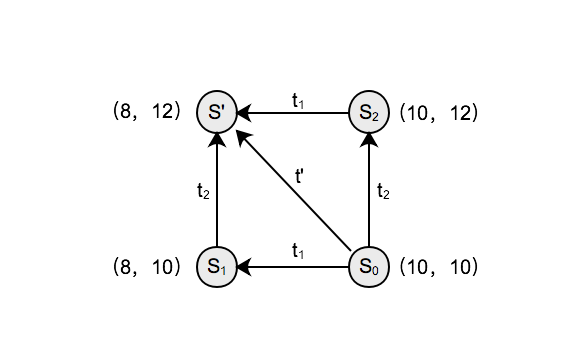
\includegraphics[width=.8\linewidth]{image/tx-deg-of-free.png}

如上图所示,假设Alice和Bob各有10元钱,系统的初始状态为$s_{0} = (10, 10)$。当Alice想给Bob转账2元时,在比特币和以太坊的模型中,可以通过一个交易${t}'$,使系统直接进入最终状态:$s_{0} \overset{{t}'}{\rightarrow}{s}'$。

而在Vite的定义中,交易${t}'$同时改变了Alice和Bob两个账户的状态,不符合单自由度的原则。因此,这个交易必须被拆分成两笔交易:

1) 表示Alice转出2元的交易$t_{1}$

2) 表示Bob转入2元的交易$t_{2}$。

这样,从初始状态到达最终状态${s}'$可以有两条不同的路径$s_{0} \overset{t_{1}}{\rightarrow} s_{1} \overset{t_{2}}{\rightarrow} {s}'$和$s_{0} \overset{t_{2}}{\rightarrow} s_{2} \overset{t_{1}}{\rightarrow} {s}'$。这两条路径分别通过中间状态$s_{1}$和$s_{2}$,这两个中间状态是最终状态${s}'$在两个账户上维度的投影。也就是说,如果只关心其中某一个账户的状态,只需要执行该账户对应的所有交易,而不需要执行其他账户的交易。

下面我们来定义如何将以太坊中的交易,拆分成Vite所要求的单自由度交易:
\begin{definition}[交易投影]
将一个自由度大于1的交易拆分成一组单自由度交易的过程,称为交易投影。一笔转账交易可以拆分成一个出账交易和一个入账交易;一个合约调用交易可以拆分成一个合约请求交易和一个合约响应交易;每个合约内部的消息调用,可以拆分成一个合约请求交易和一个合约响应交易。
\end{definition}

这样,账本中就有两种不同类型的交易,它们被称为“交易对”:
\begin{definition}[交易对]
一个入账交易或合约请求交易,统称为“请求交易”;一个出账交易或合约响应交易,统称为“响应交易”。一个请求交易和一个对应的响应交易,称为交易对。发起请求交易$t$的账户,记作$A(t)$;对应的响应交易记作:$\widetilde{t}$,该交易对应的账户,记作$A(\widetilde{t})$。
\end{definition}

根据以上定义,我们可以得出Vite中,任何两个交易之间可能存在的关系:
\begin{definition}[交易的关系]
对于两个交易$t_{1}$和$t_{2}$,可能存在如下关系:

\textbf{正交}:若$A(t_{1}) \neq A(t_{2})$,则称两个交易正交,记作$t_{1} \perp t_{2}$;

\textbf{平行}:若$A(t_{1}) = A(t_{2})$,则称两个交易平行,记作$t_{1} \parallel t_{2}$;

\textbf{因果}:若$t_{2} = \widetilde{t_{1}}$,则称两个交易具有因果关系,记作$t_{1} \rhd t_{2}$,或者$t_{2} \lhd t_{1}$。
\end{definition}

\subsection{账本定义}
定义一个账本,就是定义一个偏序集。首先,我们来定义Vite中,交易之间的偏序关系:
\begin{definition}[交易的偏序]
我们用二元关系$<$来表示两个交易的偏序关系,有:

一个响应交易,必须排在一个对应的请求交易之后:$t_{1} < t_{2} \Leftrightarrow t_{1} \rhd t_{2}$;

一个账户的所有交易,必须严格全局有序:$\forall t_{1} \parallel t_{2}$,必有:$t_{1} < t_{2}$,或$t_{2} < t_{1}$。
\end{definition}

由于建立在交易集合$T$上的偏序关系$<$满足:
\begin{itemize}
	\item 非自反性(irreflexive):$\forall t \in T$,不存在$t < t$;
	\item 传递性(transitive):$\forall t_{1},t_{2},t_{3} \in T$,若$t_{1}<t_{2},t_{2}<t_{3}$,则有$t_{1}<t_{3}$;
	\item 非对称性(asymmetric):$\forall t_{1},t_{2} \in T$,若$t_{1}<t_{2}$,则不存在$t_{2}<t_{1}$
\end{itemize}

这样,我们就可以用严格偏序集的方式来定义Vite的账本:

\begin{definition}[Vite账本]
Vite账本是给定的交易集合$T$,以及偏序关系$<$,所构成的严格偏序集。
\end{definition}

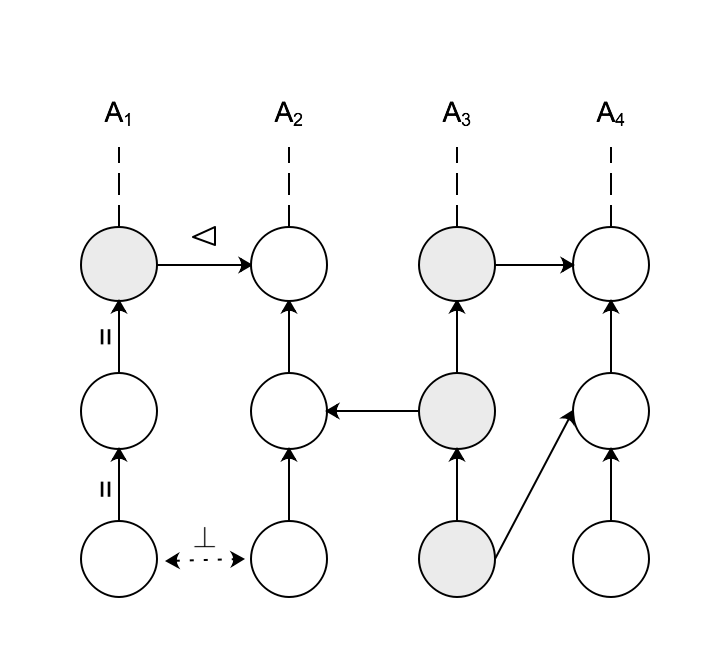
\includegraphics[width=.8\linewidth]{image/ledger.png}

一个严格偏序集,可以对应到一个DAG结构。上面所定义的Vite账本,结构类似于block-lattice。交易分为请求交易和响应交易两种,每个交易对应一个单独的区块,每个账户$A_{i}$对应一条链,一个交易对中,响应交易引用其对应的请求交易的hash。

\section{快照链}
\subsection{交易确认}
当账本发生分叉时,共识结果可能会在两个分叉账本间摇摆。例如,基于区块链结构的系统,如果节点接收到一个更长的分叉链,就会选择这个新分叉作为共识结果,而原分叉将被废弃,原分叉上的交易也会被回滚。在此类系统中,交易被回滚是一个非常严重的事件,将会导致双花(double spend)。试想,一个商家接收到一笔付款,提供了商品或服务,之后这笔付款又被撤回,商家可能会因此面临损失。因此,用户在收到一笔付款交易时,需要等待系统对这笔交易进行“确认”,以确保这笔交易被回滚的概率足够低。

\begin{definition}[交易确认]
当一个交易被回滚的概率小于一个给定的阈值$\epsilon$时,称该交易为已确认(confirmed)。
$P_{r}(t) < \epsilon \Leftrightarrow t \text{ is } \boldsymbol{confirmed}$。
\end{definition}

交易的确认是一个非常容易被混淆的概念,因为一个交易是否被确认实际上取决于隐含的置信度$1-\epsilon$。一个售卖钻石的商家和一个售卖咖啡的商家,在被双花攻击的时候,所蒙受的损失是不同的。因此,前者需要对交易设置更小的$\epsilon$。这也是比特币中确认数的本质。在比特币中,确认数表示一个交易在区块链中的深度,确认数越大,交易被回滚的概率越低\cite{nakamoto2008bitcoin}。因此,商家可以通过设置等待多少确认数,间接设定确认的置信度。

交易被回滚的概率随时间而降低,是由于账本结构中存在hash引用关系。如前文所述,当账本的设计具有较好的防篡改特性时,回滚一个交易需要重构该交易所在区块的所有后继区块。随着新的交易被不断加入账本,某个交易的后继节点也越来越多,因此,被篡改的概率也随之下降。

而block-lattice结构中,由于交易是按账户分组的,一个交易只会附加到其所属账户的账户链末端,大部分其他账户产生的交易不会自动成为该交易的后继节点。因此,采用这个结构必须合理的设计共识算法,以避免双花的隐患。

Nano采用了一个基于投票的共识算法\cite{nano},由一组用户选择的代表节点对交易进行签名,每个代表节点有一个权重,当某个交易获得的签名累计起来有足够多的权重时,就认为该交易被确认。这个算法有以下几个问题:

首先,如果需要更高的确认置信度,则需要提高投票权重的阈值,如果没有足够多的代表节点在线,就无法保证相交速度,有可能一个用户永远也搜集不到确认一个交易所必需的票数;

其次,交易被回滚的概率不随时间递减。这是因为任何时候,推翻一个历史投票的结果,所付出的成本都是一样的。

最后,历史的投票结果并没有被持久化到账本中,只保存在节点的本地存储中。当一个节点从其他节点获取账本时,没有办法可靠的量化一个历史交易被回滚的概率。

从本质上,投票的机制是一个偏中心化的解决方案。我们可以把投票结果看作是对账本状态的一个快照,这个快照会分布式的保存在网络中各个节点的本地存储中。为了拥有和区块链同样的防篡改能力,我们可以将这些快照也组织成链式结构,这就是Vite设计的核心之一——快照链\cite{snapshotchain}。

\subsection{快照链的定义}
快照链是Vite中最重要的存储结构,它的主要作用是维护Vite账本的共识。首先我们给出快照链的定义:
\begin{definition}[快照块和快照链]
一个快照块存储一个Vite账本的状态快照,状态包括:账户的余额、合约状态的Merkle root,每个账户链中最后一个块的hash。快照链是由快照块组成的链式结构,后一个快照块引用前一个快照块的hash。
\end{definition}

一个用户账户的状态包含余额和账户链最后一个块的hash;一个合约账户的状态,除了包含以上两个字段之外,还包含该账户合约状态的Merkle root hash。账户的状态的结构如下:

\begin{verbatim}
  struct AccountState {
    // 账户余额
    uint256 balance;
    // 合约状态的Merkle root
    optional uint256 storageRoot;
    // 账户链最后一个交易的hash
    uint256 lastTransaction;
  }
\end{verbatim}

快照块的结构定义如下:
\begin{verbatim}
  struct SnapshotBlock {
    // 前一个块的hash    
    uint256 prevHash;
    // 快照信息
    map<address, AccountState> snapshot;
    // 签名
    uint256 signature;
  }
\end{verbatim}

快照链中第一个快照块称为“创世快照”,保存的是账本中创世块的快照。

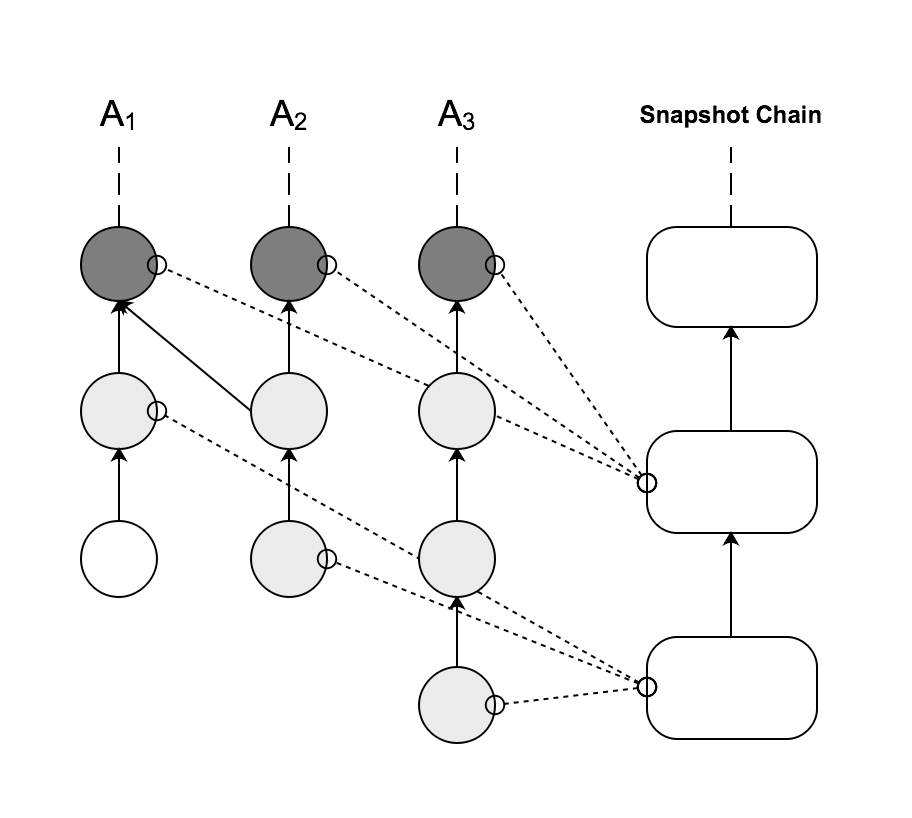
\includegraphics[width=.8\linewidth]{image/snapshotchain.png}

由于快照链中每个快照块都对应于Vite账本的唯一分叉,因此,在快照块不发生分叉的情况下,通过快照块,可以确定Vite账本的共识结果。

\subsection{快照链与交易确认}

引入了快照链之后,block-lattice结构天然的安全性缺陷就得到了弥补。攻击者想生成一个双花交易,除了要重建Vite账本中的hash引用之外,还需要重建快照链中,首次快照该交易的快照块之后的所有区块,并且需要产生一条更长的快照链。这样,攻击成本将大大提高。

在Vite中,交易的确认机制类似于比特币,定义如下:

\begin{definition}[Vite交易确认]
在Vite中,一个交易被快照链所快照,则成为该交易被确认。第一次快照该交易的快照块的深度,称为交易的确认数。
\end{definition}

在这个定义下,快照链每增长一个区块,此前所有已确认交易的确认数都增加1,双花攻击成功的概率随着快照链的不断增加而逐渐下降。这样,用户就可以根据具体的场景,通过等待不同的确认数,来定制所需的确认置信度。

快照链本身依赖一个共识算法,如果快照链发生分叉,则选取\textbf{最长的}分叉作为合法分叉。当快照链切换到新的分叉时,原有快照信息会被回滚,相当于原来对账本达成的共识被推翻,由新的共识结果取代。因此,快照链是整个系统安全性的基石,需要非常认真的对待。

\subsection{压缩存储}
由于快照链中每一个快照块都需要保存所有账户的状态,耗费的存储空间非常大,因此需要对快照链进行压缩。

\begin{center}
\begin{figurehere}
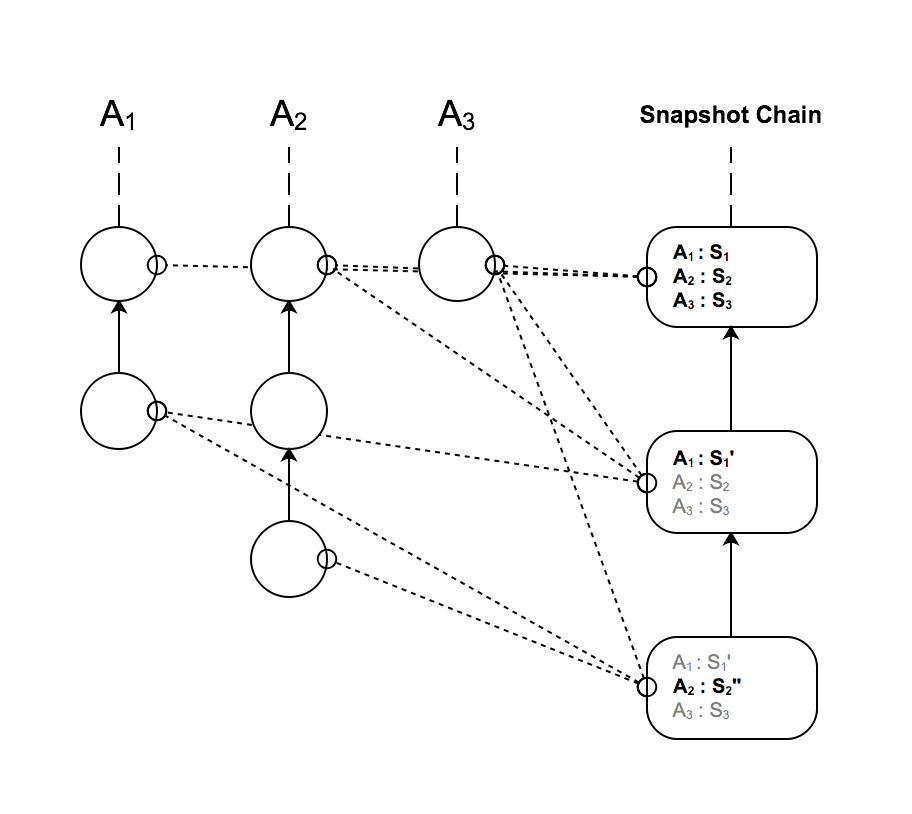
\includegraphics[width=.7\linewidth]{image/compact-snapshot.png}
\caption{压缩前的快照}
\end{figurehere}
\end{center}

压缩快照链存储空间的基本思路是利用增量存储:一个快照块只保存相比于前一个快照块发生变化的数据。如果一个账户在两个快照之间没有发生任何交易,则后一个快照块不保存该账户的数据。

要恢复快照信息,可以从前向后依次遍历快照块,将每一个快照块中的数据覆盖到当前的数据上即可。

\begin{center}
\begin{figurehere}
\centering
\tikzstyle{block} = [draw, fill=blue!20, rectangle, 
    minimum height=3em, minimum width=6em]
\tikzstyle{sum} = [draw, fill=blue!20, circle, node distance=1cm]
\tikzstyle{input} = [coordinate]
\tikzstyle{output} = [coordinate]
\tikzstyle{pinstyle} = [pin edge={to-,thin,black}]

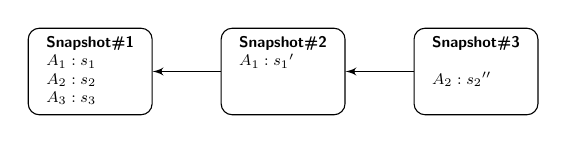
\begin{tikzpicture}[
    auto, 
    node distance=2cm,
    >=latex',
    font=\bfseries\footnotesize\sffamily,
    snapshot/.style={
		scale=0.7,
		rectangle,
		rounded corners,
		draw=black, 
		text centered,
%		text width=5cm,
		minimum height=12mm,
		fill=white
	},
	label/.style={
		scale=0.7
	}
  ]
    % We start by placing the blocks

  \node [snapshot] (snapshot2) 
 {%
 \begin{tabular}{l}
  \textbf{Snapshot\#2}\\
  $A_{1}: {s_{1}}'$\\
  \\
  \\
 \end{tabular}
 };
 
  \node [snapshot, xshift=-3.5cm] (snapshot1) 
 {%
 \begin{tabular}{l}
  \textbf{Snapshot\#1}\\
  $A_{1}: s_{1}$\\
  $A_{2}: s_{2}$\\
  $A_{3}: s_{3}$
 \end{tabular}
 };
 
 
  \node [snapshot, xshift=3.5cm] (snapshot3) 
 {%
 \begin{tabular}{l}
  \textbf{Snapshot\#3}\\
  \\
  $A_{2}: {s_{2}}''$\\
  \\
 \end{tabular}
 };
 
 \draw [draw,->] (snapshot2) -- (snapshot1);
 \draw [draw,->] (snapshot3) -- (snapshot2);

\end{tikzpicture}

\caption{压缩后的快照}
\label{fig:compact-snapshot}
\end{figurehere}
\end{center}

由于每个快照只保存在快照时刻每个账户最后的状态,不关心中间状态,无论在两个快照块之间,一个账户产生了多少交易,在快照中也只保存一份数据。因此,一个快照块最多占用$S * A$个字节。其中,$S = \text{sizeof}(s_{i})$,为每个账户状态占用的字节数,$A$是系统总账户数。如果活跃账户与总账户数的平均比例是$a$,则压缩率为$1-a$。

\section{共识}
\subsection{设计目标}
在设计共识协议时,我们需要充分考虑以下因素:
\begin{itemize}
	\item \textbf{性能}。Vite的首要设计目标是快速,为确保系统具有高吞吐、低延迟的性能表现,我们需要采用具有更高相交速度的共识算法。
	\item \textbf{扩展性}。Vite是一个公共平台,向所有去中心化应用开放,因此,扩展性也是一个重要的考量因素。
	\item \textbf{安全性}。虽然Vite的设计理念不是追求极致的安全性,但仍然需要确保足够的安全性底线,有效防范各类攻击。
\end{itemize}

对比现存的一些共识算法,PoW的安全性更好,在恶意节点低于50\%的情况下可以确保达成共识。但PoW的相交速度较慢,无法满足性能要求;
PoS及其变种算法去掉了求解数学难题的步骤,提高了相交速度和单次攻击成本,降低了能源消耗。但PoS的扩展性仍然较差,而且Nothing at Stake问题\cite{problems}较难解决;
BFT系列算法在安全性和性能方面有较好表现,但其扩展性是一个问题,通常比较适合于私有链或联盟链;
DPoS\cite{dpos}系列算法通过限制生成区块的权限,有效降低了伪分叉率,在性能和扩展性方面表现良好。相应的,DPoS在安全性方面稍有牺牲,需要保证恶意节点数不超过1/3\cite{dpos2}。

综合来看,DPoS算法在性能、扩展性方面有比较明显的优势,因此,我们选择DPoS作为Vite共识协议的基础,并在其基础上进行适当扩展,通过分层共识协议和异步模型,进一步提高平台的整体性能。

\subsection{分层共识}
Vite的共识协议称为HDPOS(Hierarchical Delegated Proof Of Stake)。基本思想是对共识函数$\Phi$进行函数分解(functional decomposition):
\begin{equation}
\begin{split}
\Phi(l_1,l_2,\dots,l_n) = \Psi(\Lambda_1(l_1,l_2,\dots,l_n), \\
\Lambda_2(l_1,l_2,\dots,l_n),\dots \\
\Lambda_m(l_1,l_2,\dots,l_n))
\end{split}
\end{equation}

其中,$\Lambda_i: 2^L \rightarrow L$,称为局部共识函数,返回的结果称为局部共识;$\Psi: 2^L \rightarrow L$,称为全局共识函数,它从一组候选的局部共识中选取一个唯一结果,作为最终的共识结果。

这样拆分之后,整个系统的共识变成了两个独立的过程:
\begin{labeling}{alligator}
\item [局部共识] 生产用户账户或合约账户中的请求交易和响应交易对应的区块,并写入账本;
\item [全局共识] 对账本中的数据进行快照,生产快照块。如果账本有分叉,则选择其中一个。
\end{labeling}

\subsection{区块生产权和共识组}
那么,谁有权生产账本中的交易区块和快照链中的快照块,采用什么共识算法达成共识呢?

由于Vite的账本结构是按账户不同组织成多条账户链的,我们可以方便的按账户的维度来限定账本中区块的生产权,再加上快照块的生产权归属于单独的一组用户。这样,我们就可以将若干条账户链或快照链归入一个共识组,在共识组内部,用统一的方式来生产区块并达成共识。

\begin{definition}[共识组]
共识组是一个元组$(L, U, \Phi, P)$,描述了账本的一部分或快照链的共识机制。其中,$L \in A \vert \{ A_s \}$,表示账本中属于该共识组的一条或若干条账户链,或者是快照链;$U$表示拥有$L$指定的链上区块生产权的用户;$\Phi$指定该共识组的共识算法;$P$指定共识算法的参数。
\end{definition}

在这样的定义下,用户可以根据需要,灵活的设置共识组,并选择不同的共识参数。下面我们对不同的共识组加以详细说明:

\subsubsection{快照共识组}
快照链所在的共识组称为快照共识组,这是Vite中最重要的一个共识组。快照共识组的共识算法$\Phi$对应分层模型中的$\Psi$,采用DPoS算法。由参数$P$指定代理节点数和出块间隔。

例如,可以采用25个代理节点,以10秒为间隔生产快照块。这样可以保证交易的确认速度足够快,一个交易达到6次确认最多需要等待60秒。

\subsubsection{私有共识组}
私有共识组只适用于账本中交易区块的生产,属于私有共识组的账户链,区块只能由账户的私钥拥有者来生产。默认情况下所有用户账户都属于私有共识组。

私有共识组的最大好处是降低分叉概率。因为只有一个用户有权生产区块,发生分叉的唯一可能是用户主动发起双花攻击,或程序发生错误。

私有共识组的缺点是用户节点必须在线,才能打包交易。这对合约账户来说不太适合,一旦合约拥有者的节点失效,没有其他节点可以代替它生产合约的响应交易,相当于降低了dApp的服务可用性。

\subsubsection{委托共识组}
在委托共识组中,由一组指定的代理节点,通过DPoS算法,代替用户打包账户链上的交易。无论是用户账户还是合约账户,都可以加入委托共识组。用户可以设置一组单独的代理节点,建立一个新的委托共识组。Vite中还有一个默认的委托共识组,来帮助所有未单独建立委托共识组的账户打包交易,这个共识组也称为\textbf{公共共识组}。

委托共识组适合于大部分合约账户,因为合约账户的交易大部分都是合约响应交易,相比于用户账户的收款交易,需要更高的可用性和更低的延迟。

\subsection{共识的优先级}
在Vite协议中,全局共识的优先级高于局部共识。当局部共识发生分叉的时候,以全局共识选择的结果为准。也就是说,一旦全局共识选定局部共识的一个分叉作为最终结果,即使未来账本中某个账户链出现更长的分叉,也不会使全局共识结果回滚。

在实现跨链协议的时候,这个问题需要格外注意。由于某个目标链可能发生回滚,映射该链的中继合约对应的账户链也需要随之回滚。这个时候,如果中继链的局部共识已经被全局共识采纳,是无法完成回滚的,可能会导致中继合约和目标链的数据不一致。

避免这个问题的方法是在共识组参数$P$中设置一个\textit{delay}参数,指定快照共识组在局部共识完成后\textit{delay}个区块之后,才开始进行快照。这样将大大降低中继合约不一致的概率,但也无法完全避免。在中继合约的代码逻辑中,还需要对目标链回滚的情况做单独处理。

\subsection{异步模型}
为了进一步提高系统吞吐,我们需要在共识机制上支持更完善的异步模型。

一个交易的生命周期包括:交易发起、交易写入、交易确认。为了提高系统的性能,我们需要将这三个步骤设计成异步模式。这是因为在不同的时刻,用户发起交易的数量是不同的,而系统处理交易写入和确认交易的速度相对固定。异步模式有利于削平波峰波谷,从而提高系统的整体吞吐能力。

比特币和以太坊等系统的异步模型比较简单:将所有用户发起的交易放入一个未确认交易池中,当矿工将其打包到一个区块中,该交易同时完成了写入和确认,当区块链继续增长时,该交易最终到达预设的确认置信度。

这个异步模型存在两个问题:
\begin{itemize}
	\item 交易在未确认状态下没有持久化到账本。未确认的交易是不稳定的,没有参与共识,也无法防止交易重复发送;
	\item 交易的写入和确认之间没有异步机制。交易只有在确认时才写入账本,写入速度受制于确认速度。
\end{itemize}

Vite协议建立了更完善的异步模型:首先,将交易拆分成基于“请求-响应”模式的交易对,无论是转账还是合约调用,当一个请求交易被写入账本,则代表该交易被成功发起。另外,交易被写入账本和确认也是异步的。交易可以先被写入Vite的DAG账本中,不会被确认过程阻塞。交易的确认通过快照链来完成,快照的动作也是异步进行的。

这是一个典型的生产者-消费者模型,在交易的生命周期中,无论上游的生产速率如何变动,下游都可以以恒定的速率消化待处理的交易,从而充分利用平台资源,提高了系统的吞吐。

\section{虚拟机}
当前以太坊生态相对较为成熟,已经有大量基于EVM的智能合约运行在其上。为方便既有的存量应用无缝迁移到新平台,Vite的智能合约虚拟机将提供EVM兼容性。由于Vite的账本结构和以太坊不同,一些EVM指令的语义需要重新定义。此外,我们将针对EVM和Solidity的一些不足做一些改进,从而提高Vite对智能合约的支持能力。

\subsection{标准库}
在以太坊上开发智能合约的开发者,经常被Solidity缺乏标准库的问题所困扰。例如,路印协议中的环路验证必须在链外执行,其中一个重要原因就是Solidity没有提供浮点运算功能,尤其是求浮点数的n次方根\cite{loopring}。

在EVM中,可以通过DELEGATECALL指令来调用一个预先部署的合约,实现库函数的功能。以太坊也提供了几个预编译合约(Precompiled Contract),主要是几个Hash运算。但这些功能都太过简单,无法满足复杂的应用需求。

因此,我们将在Vite中扩展Solidity的功能,提供一系列标准合约库,例如:字符串处理、浮点运算、基本数学运算、容器、排序等。

基于性能考虑,这些标准库将以本地扩展(Native Extension)的方式实现,将大部分运算内置到Vite本地代码中,只在EVM代码中通过DELEGATECALL指令来完成方法的调用。

标准库可以根据需要不断扩展,但由于整个系统的状态机模型是确定性的,因此无法提供类似于随机数之类的功能。同以太坊类似,我们可以通过快照链的hash来模拟伪随机数。

\subsection{观察者模式}
在以太坊中,智能合约是由交易驱动的,合约的执行只能通过用户主动发起一个交易来触发。而在有些应用中,需要根据一些事件自动触发合约的执行,因此,Vite提供了对观察者(Observer)模式的支持。

在Vite中,一个观察者(Observer)可以订阅一个被观察对象(Observable)上的事件,并通过回调方法来定义事件响应逻辑。通常,观察者是一个智能合约,被观察对象可以是智能合约,也可以是快照链。被观察对象会维护所有订阅它的观察者列表,当一个事件发生时,例如快照链的高度每次增长时,就会依次触发订阅列表中观察者的回调方法。这个动作是由生产被观察对象区块的节点来执行,执行的结果由其他节点验证。

为了保证Vite交易定义中的单自由度原则不被打破,每执行一次事件回调,都需要向账本中显式加入一个交易对。请注意,这类交易不是由用户发起的,而是由Vite系统自动产生。为了确保回调交易能够在事件发生时可靠生成,观察者模式只适用于快照共识组和公共共识组,不支持私有共识组和用户定制的委托共识组。

\subsection{燃料}

\subsection{同步语义和异步语义}

\section{经济模型}
\subsection{配额}
由于Vite是一个通用的dApp平台,部署在其上的智能合约功能各不相同,每一个不同的智能合约,对吞吐和延迟的需求也不同。即使是同一个智能合约,在不同阶段对性能的要求也不同。

在以太坊的设计中,每一个交易在发起时需要指定一个gas price,从而与其他交易竞争写入账本的机会。这是一个典型的竞价模型,原则上可以通过价格有效调控供给和需求的平衡。但由于用户在出价之前,很难量化当前的供需情况,也无法预测其他竞争者的出价,很容易发生市场失灵(market failure)。而且,每次出价所竞争的资源都是针对一个交易的,没有一个按账户维度对资源进行合理配置的协议。
$$
TPS_{n} =  \frac{10}{S\cdot(H_{n}  -  H_{n-9} + 1)}
$$
\section{内置协议}

\section{跨链}

\section{总结}

Vite的特点总结如下:

\begin{itemize}
	\item 特点一。
\end{itemize}

\section{致谢}
致谢部分。

\end{multicols}

\bibliography{vite}
\bibliographystyle{unsrt}

\end{document}
